%
% Updated 12-31-2019
%

\usepackage{booktabs}
\usepackage[nottoc,numbib]{tocbibind}
\usepackage{amsmath}
\usepackage{color}
\usepackage{amsbsy}
\usepackage[normalem]{ulem}
\usepackage{cancel}
\usepackage{geometry}
\usepackage{framed}
\usepackage[fit]{truncate}
\usepackage{fancyhdr}


\definecolor{WhiteSmoke}{RGB}{245, 245, 245} % #F5F5F5
\definecolor{Silver}{RGB}{192, 192, 192} % #C0C0C0
\definecolor{Grey}{RGB}{128, 128, 128} % #808080
\colorlet{shadecolor}{WhiteSmoke}
\colorlet{framecolor}{Silver}



%\usepackage[svgnames]{xcolor} There is a conflict with xcolor. Defining the needed colors from xcolor

\colorlet{shadecolor}{Silver} %Probably too dark...

\usepackage{float}
\usepackage{caption}
\usepackage{url}
\usepackage{makeidx}


\newgeometry{inner=1.25in,outer=0.75in,top=1in,bottom=1in}
\definecolor{whitesmoke}{RGB}{245,245,245}
\definecolor{silver}{RGB}{192,192,192}
\definecolor{Grey}{RGB}{128,128,128}
\colorlet{shadecolor}{whitesmoke}
\colorlet{framecolor}{silver}
\definecolor{purple}{RGB}{76,0,153}

% % make code-output smaller
% \DefineVerbatimEnvironment{Highlighting}{Verbatim}{fontsize=\tiny,commandchars=\\\{\}}
% 

% make console-output smaller:
%  \makeatletter
% \def\verbatim{\small\@verbatim \frenchspacing\@vobeyspaces \@xverbatim}
% \makeatother

%\setlength{\parindent}{0pt} % Default is 0pt. Use \indent to indent targeted paragraphs

%Making my own indent command
\renewcommand{\indent}{\hspace{15pt}}

%\setlength{\parskip}{0pt}


\setlength{\OuterFrameSep}{0pt}
\setlength{\FrameRule}{1.5pt}
\makeatletter
\def\preto{\@verbatim}{\topsep=-10pt \partopsep=-10pt }
\makeatother

% Adjust verbatim shade environments
\renewenvironment{Shaded}{%
\setlength{\FrameRule}{1.5pt}
\def\FrameCommand{\fboxrule=\FrameRule\fboxsep=5pt
                  \fcolorbox{framecolor}{shadecolor}}%
\MakeFramed {\FrameRestore}}%
{\endMakeFramed}



%Change third level of itemize to an open circle instead of an asterisk
\renewcommand{\labelitemiii}{$\circ$}

%Change fourth level of itemize to an dash instead of an asterisk
\renewcommand{\labelitemiv}{\textendash}

\newcommand{\BD}{\boldsymbol{\Delta}}

\renewcommand*{\maketitle}{%
\begin{titlepage}
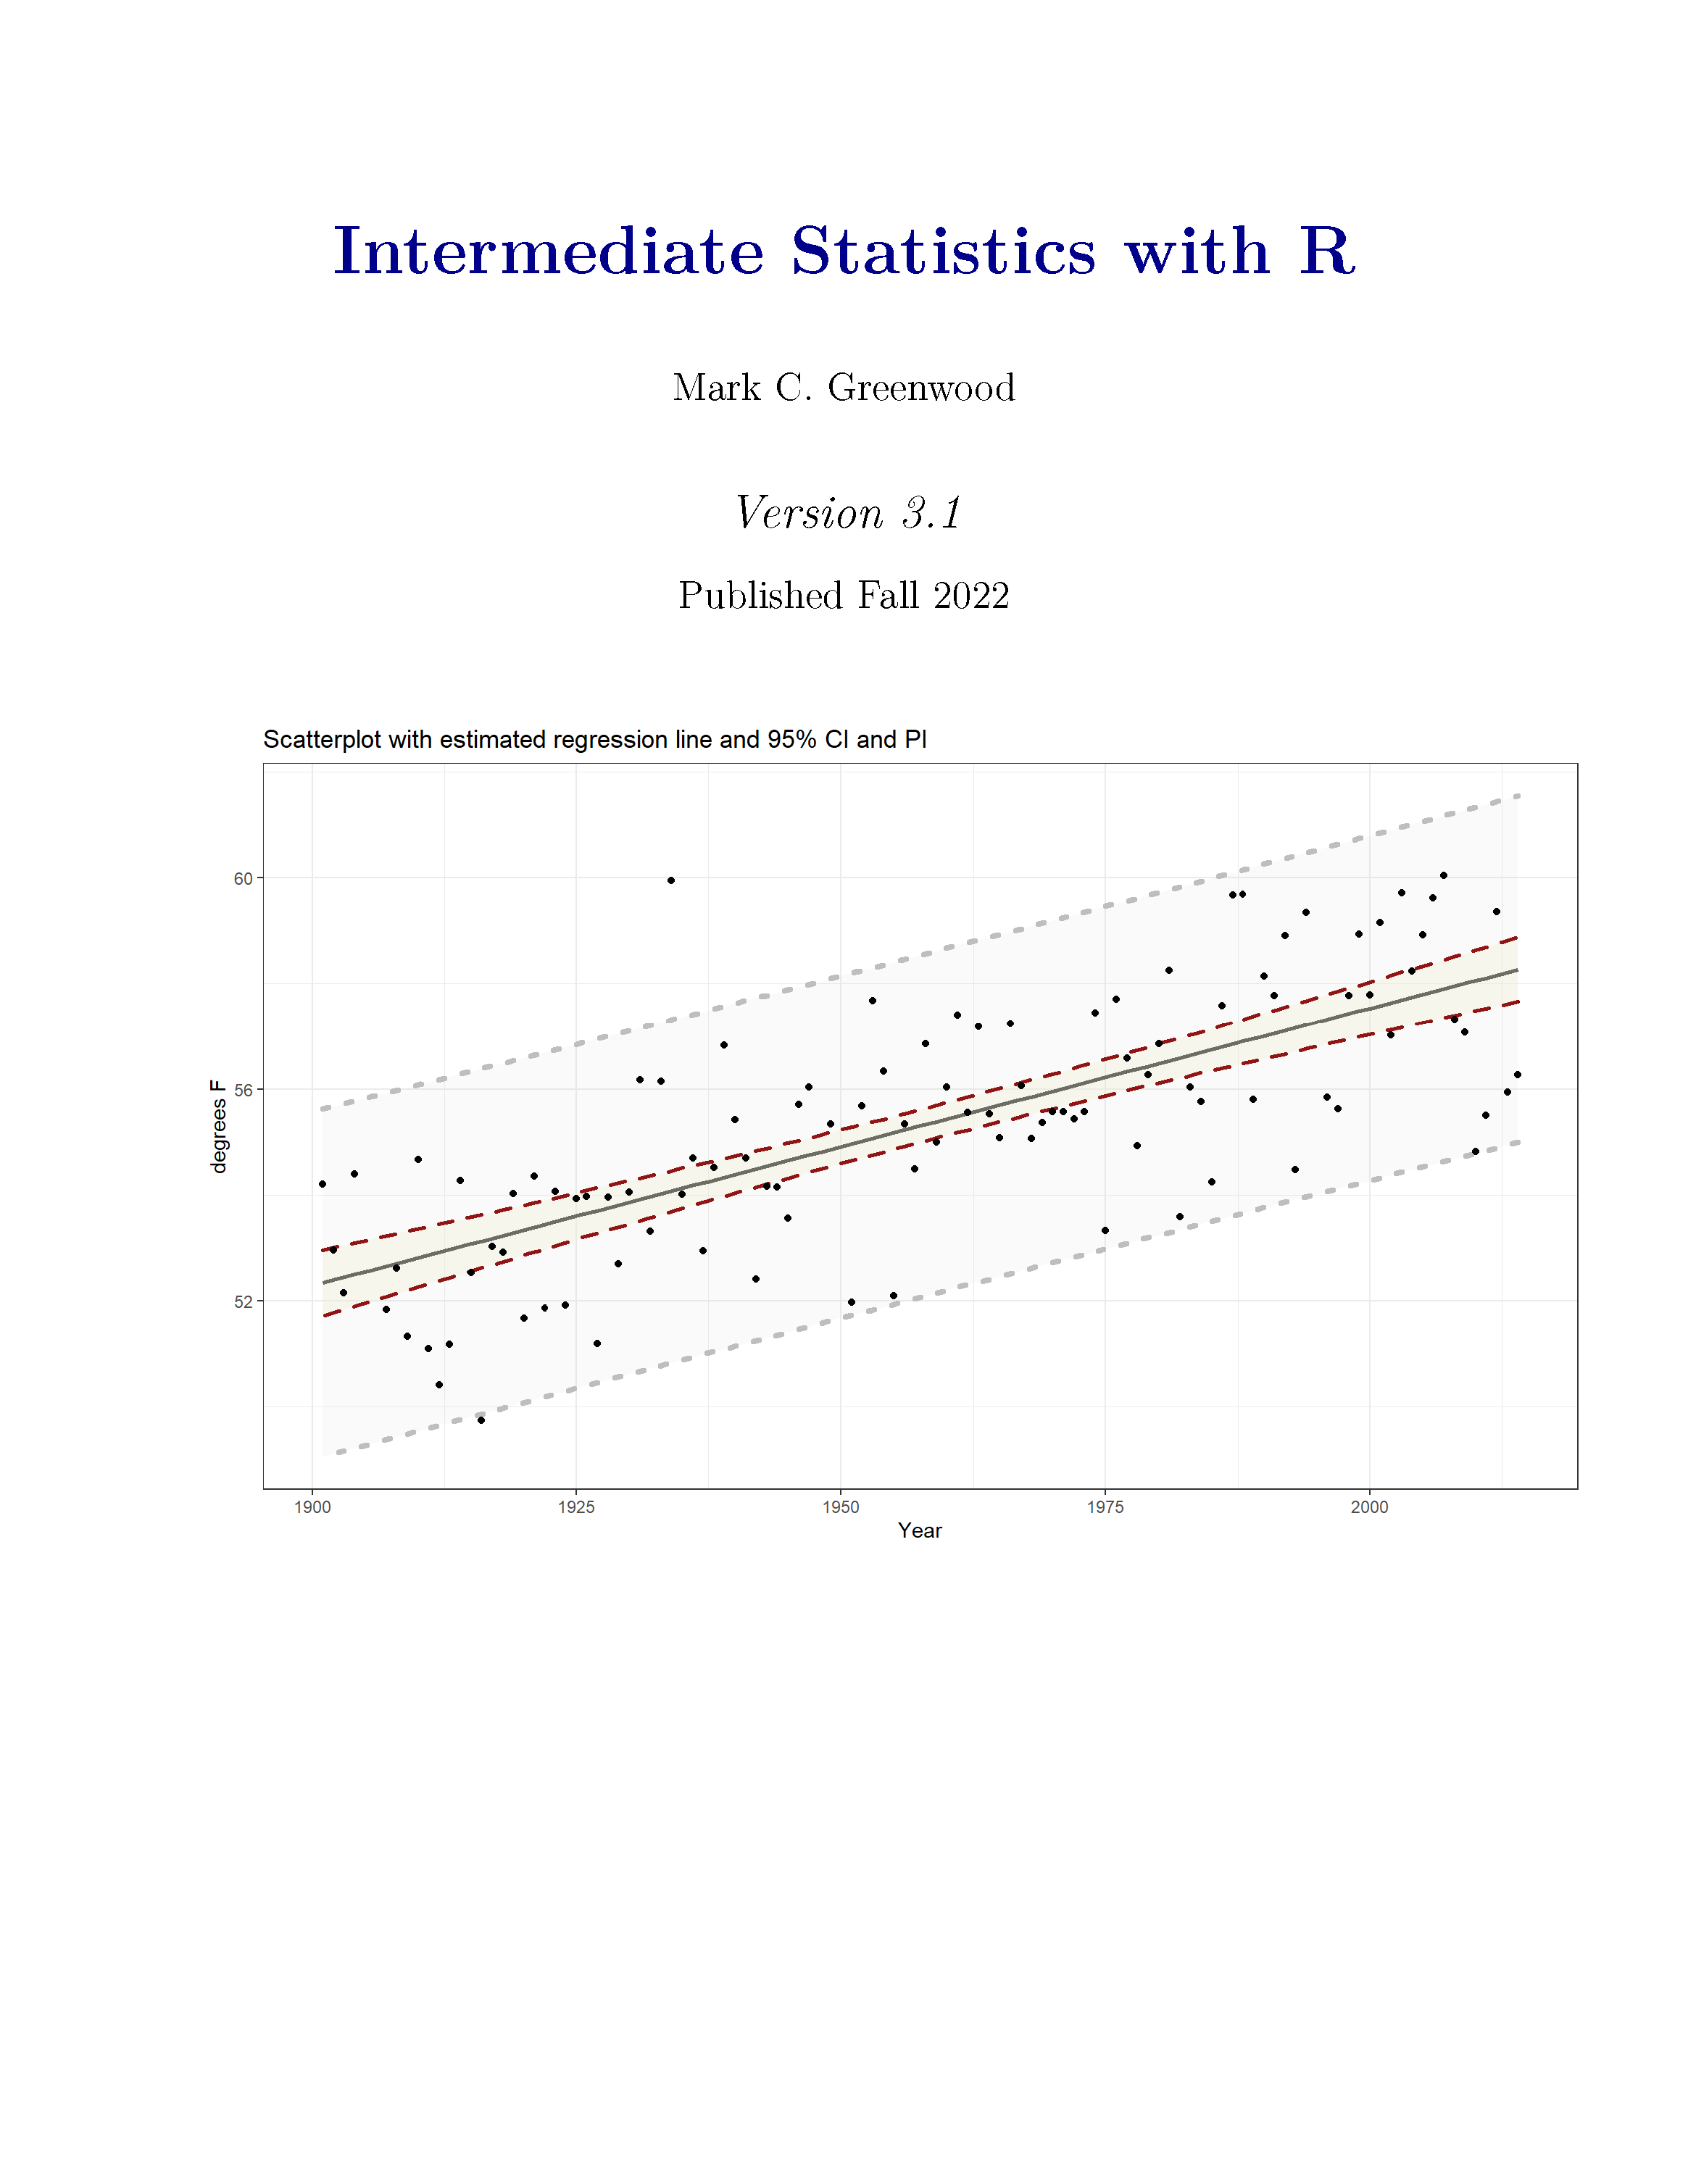
\includegraphics{titlepage_summer_2022.pdf}
\end{titlepage}
}

\pagestyle{fancy}
\fancyhf{} % --- clear all fields
\fancyhead[LE, RO]{\thepage} %Add page number to outside of page in header
\fancyhead[RE]{\leftmark}
\fancyhead[LO]{\truncate{0.95\headwidth}{\rightmark}}

% Uncomment below to make an index (only for pdf version).
% Will also need to figure out how to make the bookmark jump to the Index
% and not the Bibliography in the pdf file
\makeindex